\section{Results}
\label{sec:results}

The main experiment comprises \NRuns{} runs (\NEdTypes{} ED types, all policies, \Reps{} replications) with on average \PatientsPerRunMean{} patients per run in the observation window. All automated checks passed: every observed patient departed in every run, every overall mean lay within the range of its group means, and runs shared between experiments gave identical results.

\subsection{Verification and Validation}

In the community, medium-load, pooled ED, the stage-to-stage transition frequencies recovered from the event log differ from those implied by the generator by at most \TransMaxDiffGen{}, and the pathway shares by at most \PathMaxDiffGen{}. The process logic therefore reproduces the intended pathways. Compared with the published pathway table, transition frequencies differ by at most \TransMaxDiffPub{}; the difference comes from the CTAS-specific tilt toward more diagnostic steps for higher-acuity patients, which the published table, pooled over all patients, does not show.

Table~\ref{tab:face} reports time intervals for the same ED at the three load levels under the default policy. The 90th percentile of LOS for discharged CTAS~4 patients ranges from \FvLosCtasFourPNinetyLow{} hours at low load to \FvLosCtasFourPNinetyHigh{} hours at high load, which brackets the national Canadian value of \CihiNonAdmPNinety{} hours for less urgent discharged visits in 2025--2026 \cite{CIHI2026_NACRS}. The model is less congested than the average Canadian ED in other respects. Median door-to-physician times are below half an hour at all load levels, and the 90th percentile of LOS for admitted patients is about \FvLosAdmPNinetyHigh{} hours at high load, far below the national value of \CihiAdmPNinety{} hours, because boarding in the core design is short (mean \BoardLowMean{} minutes, at the lower end of reported provincial medians of \ProvBedWaitLow--\ProvBedWaitHigh{} hours \cite{Li2023_EDOvercrowdingCADTH}). The high boarding level in the sensitivity analysis moves the model toward the national situation. These comparisons support the use of the model for comparing policies; they do not make it a forecast of any particular ED.

\begin{table}[!t]
\centering
\caption{Face validity: community ED, pooled configuration, default policy, \Reps{} replications per load level.}
\label{tab:face}
\footnotesize
\begin{adjustbox}{max width=\linewidth}\begin{tabular}{lrrr}
\toprule
Measure (h unless stated) & Low & Medium & High \\
\midrule
Door to physician, median & 0.2 & 0.2 & 0.4 \\
Door to physician, P90 & 0.4 & 0.8 & 3.4 \\
LOS discharged, median & 1.5 & 1.6 & 2.1 \\
LOS discharged, P90 & 3.2 & 3.7 & 6.2 \\
LOS CTAS 4, P90 & 3.5 & 4.7 & 8.9 \\
LOS admitted, median & 4.9 & 5.1 & 5.4 \\
LOS admitted, P90 & 9.1 & 9.4 & 10.3 \\
Physician utilisation & 0.70 & 0.80 & 0.90 \\
Space utilisation & 0.54 & 0.67 & 0.85 \\
\bottomrule
\end{tabular}\end{adjustbox}
\end{table}

\subsection{Policy Fidelity of Similarity Rules (RQ4)}

Table~\ref{tab:fidelity} reports fidelity in the three medium-load fast-track EDs. The settings that satisfy Propositions~\ref{prop:lex} and~\ref{prop:route} reproduced their reference rules exactly: in every replication they chose the same patient at every one of about \FidDecisionsPerRun{} queue decisions per run, Kendall's $\tau$ between the two queue orders was 1, and the event logs were identical, so all outcomes were identical as well.

The two settings that violate condition (\ref{eq:lexcond}) behaved differently. With equal weights on CTAS and service class, the similarity rule chose the same patient as CTAS-SPT at \FidSimrepNearAgree\% of decisions (between \FidSimrepNearAgreeMin\% and \FidSimrepNearAgreeMax\% across the three acuity mixes; $\tau=\FidSimrepNearTau$). The SIM rule, which is often described as ``acuity first, then quick patients'', agreed with CTAS-SPT at only \FidSimAgree\% of decisions ($\tau=\FidSimTau$). Yet the outcomes of SIM and CTAS-SPT were close: mean LOS differed by \FidSimDLos\% and RATP by \FidSimDRatp{} on average. A comparison of average outcomes would therefore suggest that SIM ``is'' CTAS-SPT, while at the level of individual decisions the two rules disagree about half of the time. The disagreement matters for patients: under SIM a CTAS~3 patient with a short expected service can be seen before a CTAS~2 patient with a long one, which CTAS-SPT never allows.

At the routing level, two-target similarity routing with weight on CTAS only reproduced CTAS streaming exactly. Similarity routing with the SIM weights agreed with prediction streaming on \FidStreamSimAgree\% of patients, and the outcomes differed strongly because the two rules send very different patients to the second area (Section~\ref{sec:res:mech}).

\begin{table*}[!t]
\centering
\caption{Fidelity of similarity settings to reference rules (medium-load fast-track EDs, three acuity mixes, \FidReps{} replications each). Agreement: share of decisions (queue) or patients (routing) for which both rules make the same choice. $\Delta$ mean LOS: similarity setting minus reference rule, with 95\% confidence half-width.}
\label{tab:fidelity}
\footnotesize
\begin{adjustbox}{max width=\linewidth}\begin{tabular}{llrrrrr}
\toprule
Similarity setting & Reference rule & Prop. & Agreement (\%) & Kendall $\tau$ & Identical logs (\%) & $\Delta$ mean LOS (\%) \\
\midrule
$w=(1,0,\dots)$ & CTAS & 2 (holds) & 100.0 & 1.00 & 100 & $0$ \\
$w_A=0.85, w_B=0.15$ & CTAS-SPT & 2 (holds) & 100.0 & 1.00 & 100 & $0$ \\
$w_A=0.85, w_C=0.15$ & CTAS-PD & 2 (holds) & 100.0 & 1.00 & 100 & $0$ \\
routing, $w=(1,0,\dots)$ & CTAS streaming & 3 (holds) & 100.0 & -- & 100 & $0$ \\
$w_A=w_B=0.25$ & CTAS-SPT & 2 (fails) & 78.0 & 0.80 & 0 & -0.7 $\pm$ 0.1 \\
SIM weights & CTAS-SPT & 2 (fails) & 53.2 & 0.39 & 0 & -0.2 $\pm$ 0.2 \\
similarity routing & prediction streaming & 3 (fails) & 70.4 & -- & 0 & -39.2 $\pm$ 12.8 \\
\bottomrule
\end{tabular}\end{adjustbox}
\end{table*}

\subsection{Best Policy by ED Type (RQ1)}

Fig.~\ref{fig:heatmap} shows, for each ED type, the policy with the lowest mean RATP and the policy with the lowest mean LOS, together with the number of policies that cannot be distinguished from the best at the 95\% level. The best policy is usually distinguishable from most others; the median number of policies tied with the best (including the best itself) is \MedianTiedRatp{} for RATP and \MedianTiedLosAllMean{} for mean LOS.

\begin{figure*}[!t]
\centering
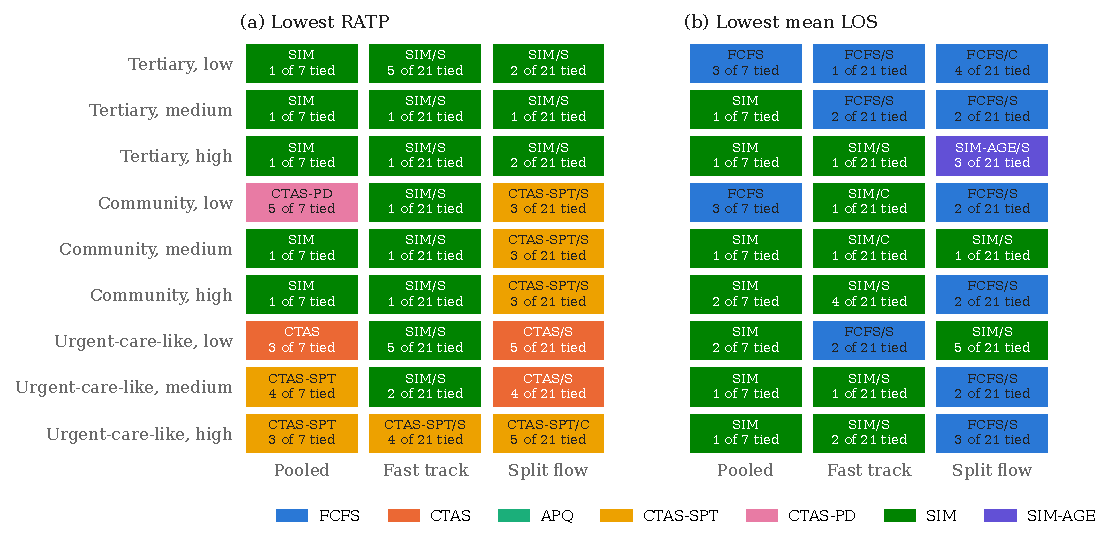
\includegraphics[width=0.92\textwidth]{figures/fig_best_policy_heatmap.pdf}
\caption{Best policy by ED type for (a) RATP and (b) mean LOS. Cell colour shows the queue rule; the label gives the policy (queue rule/routing rule: C CTAS streaming, P prediction streaming, S similarity routing) and the number of policies whose paired difference from the best is not significant at the 95\% level (\Reps{} replications).}
\label{fig:heatmap}
\end{figure*}

The best policy differs across ED types. For RATP, \NDistinctBestRatp{} different policies are best somewhere, built on \NDistinctBestQueueRatp{} different queue rules: SIM is best in \NBestRatpSim{} ED types, CTAS-SPT in \NBestRatpCtasSpt, CTAS in \NBestRatpCtas{} and CTAS-PD in \NBestRatpCtasPd. The pattern follows the acuity mix. In tertiary EDs, SIM is best in every configuration and load level; in urgent-care-like EDs, rules that keep strict CTAS order (CTAS and CTAS-SPT) are best in every configuration and load level except the medium- and low-load fast track; community EDs lie in between, with the configuration deciding. For mean LOS, SIM is best in \NBestLosAllMeanSim{} ED types and FCFS in \NBestLosAllMeanFcfs, mostly at low load and in split flow, where queues are short and the order matters little. The default policy is the best policy for RATP in \DefaultIsBestRatp{} of the \NEdTypes{} ED types and for mean LOS in \DefaultIsBestLosAllMean.

In the two-area configurations the routing rule matters at least as much as the queue rule. Similarity routing is part of the best policy for RATP in \NBestRouteRatpStreamSim{} of the \NTwoAreaTypes{} two-area ED types and for mean LOS in \NBestRouteLosAllMeanStreamSim; prediction streaming is never best. Relative to the default policy, the best policy lowers mean RATP by \BestVsDefaultRatpMean\% on average (up to \BestVsDefaultRatpMax\%), with a significant difference in \BestVsDefaultRatpNSig{} of \NEdTypes{} ED types, and mean LOS by \BestVsDefaultLosAllMeanMean\% on average (up to \BestVsDefaultLosAllMeanMax\%; significant in \BestVsDefaultLosAllMeanNSig{} ED types). Table~\ref{tab:best} in the Appendix lists the values for every ED type.

\subsection{Cost of a Single Policy for All ED Types (RQ2)}

Table~\ref{tab:regret} reports, for each measure, the single policy with the smallest mean regret across the \NEdTypes{} ED types, and the regret of the default policy. Fig.~\ref{fig:regret} shows the regret per ED type for the two primary measures.

\begin{table*}[!t]
\centering
\caption{Regret of one-size-fits-all policies across the \NEdTypes{} core ED types: mean and maximum relative regret, and number of ED types with regret above 10\%. The best single policy is chosen separately for each measure.}
\label{tab:regret}
\footnotesize
\begin{adjustbox}{max width=\linewidth}\begin{tabular}{llrrrrrr}
\toprule
 & \multicolumn{4}{c}{Best single policy (one size fits all)} & \multicolumn{3}{c}{Default (CTAS/C)} \\
\cmidrule(lr){2-5}\cmidrule(lr){6-8}
KPI & Policy & Mean (\%) & Max (\%) & $>10\%$ & Mean (\%) & Max (\%) & $>10\%$ \\
\midrule
RATP & CTAS-SPT/S & 2.8 & 13.5 & 1 & 15.6 & 43.8 & 17 \\
Mean LOS & SIM/S & 0.3 & 3.5 & 0 & 4.8 & 18.1 & 4 \\
AWT & APQ/S & 8.2 & 50.1 & 9 & 54.9 & 209.5 & 24 \\
P90 door to physician & SIM/S & 1.7 & 26.5 & 1 & 52.4 & 150.3 & 25 \\
P95 door to physician, CTAS 2 & CTAS/S & 2.3 & 25.1 & 2 & 4.2 & 11.2 & 4 \\
P95 door to physician, CTAS 5 & FCFS/C & 0.0 & 0.0 & 0 & 388.1 & 1093.5 & 27 \\
\bottomrule
\end{tabular}\end{adjustbox}
\end{table*}

\begin{figure}[!t]
\centering
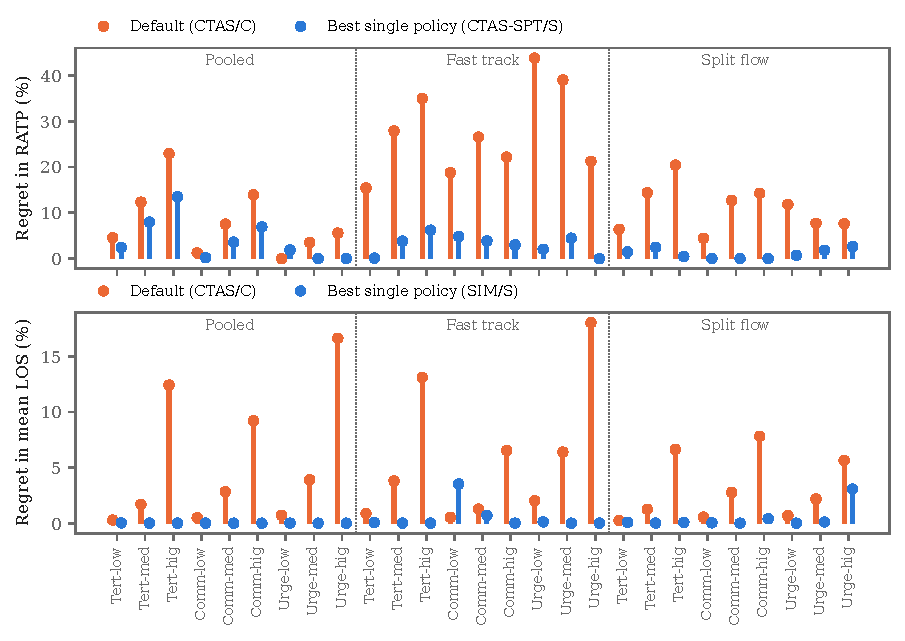
\includegraphics[width=\columnwidth]{figures/fig_regret.pdf}
\caption{Regret per ED type of the default policy and of the best single policy, for RATP (top) and mean LOS (bottom). ED types are grouped by configuration; labels give acuity mix and load.}
\label{fig:regret}
\end{figure}

Three findings stand out. First, the default policy CTAS/C is far from the best in many ED types: its mean regret is \DefaultRatpMeanRegret\% for RATP (above 10\% in \DefaultRatpNGtTen{} ED types, at most \DefaultRatpMaxRegret\%), \DefaultLosAllMeanMeanRegret\% for mean LOS, \DefaultAwtMeanRegret\% for AWT and \DefaultPiaAllPninezeroMeanRegret\% for the 90th percentile of door-to-physician time. Its regret is largest in fast-track EDs, where CTAS streaming leaves second-area physicians with spare capacity while Main-area patients wait.

Second, for any one measure, a well-chosen single policy comes close to the best in most ED types. For RATP the best single policy is \OsfaRatpPolicy, with mean regret \OsfaRatpMeanRegret\% and maximum \OsfaRatpMaxRegret\% (\OsfaRatpWorstType); for mean LOS it is \OsfaLosAllMeanPolicy, with mean regret \OsfaLosAllMeanMeanRegret\% and maximum \OsfaLosAllMeanMaxRegret\%. Standardizing on a good policy therefore costs little on the measure for which it was chosen.

Third, the best single policy depends on the measure. \OsfaRatpPolicy{} is best for RATP, \OsfaLosAllMeanPolicy{} for mean LOS, \OsfaAwtPolicy{} for AWT, \OsfaPiaCtastwoPninefivePolicy{} for the 95th percentile of door-to-physician time of CTAS~2 patients, and \OsfaPiaCtasfivePninefivePolicy{} for the 95th percentile of CTAS~5 patients. The cross-regrets are moderate between the two primary measures (\OsfaRatpPolicy{} has a mean LOS regret of \CrossRatpOnLosAllMean\%; \OsfaLosAllMeanPolicy{} a mean RATP regret of \CrossLosAllMeanOnRatp\%), but large for the tails: every rule that gives priority by acuity or predicted service lengthens the longest waits of CTAS~5 patients several times over relative to FCFS (Section~\ref{sec:res:mech}). A health system that standardizes on one policy is therefore choosing which objective to favour as much as which policy to use.

\subsection{Mechanisms and Trade-Offs}
\label{sec:res:mech}

The advantage of similarity routing comes from how many and which patients it sends to the second area. CTAS streaming sends \ShareSecondStreamCtasMin--\ShareSecondStreamCtasMax\% of patients to the second area, depending on the acuity mix; similarity routing sends \ShareSecondStreamSimMin--\ShareSecondStreamSimMax\%, because it also sends CTAS~3 patients with simple predicted profiles. With the CTAS queue rule, this lowers the mean door-to-physician time of CTAS~3 patients by \SimVsCtasRouteCtasThreeWait\% on average across the two-area ED types and raises that of CTAS~4 patients by \SimVsCtasRouteCtasFourWait\%, and it lowers RATP in \SimVsCtasRouteNBetterRatp{} of \NTwoAreaTypes{} ED types. The gain thus comes from moving waiting from a level with a shorter target to a level with a longer one, which RATP rewards, and from using second-area capacity that CTAS streaming leaves idle.

Prediction streaming, as defined here, sends only patients with a predicted quick discharge to the second area and keeps every other patient, including most CTAS~4--5 patients who need tests, in the Main area. When capacity is split by acuity, as it is in our sizing and in many EDs, this overloads the Main area. In \NOverloadedTypes{} ED types (\OverloadedTypesList) prediction streaming kept Main-area utilization at or above \OverloadThreshold, so that queues grew throughout the run; we report these cases as overloaded rather than interpret their averages. Prediction streaming had the highest mean LOS of all policies in \NWorstLosPredStream{} of the \NTwoAreaTypes{} two-area ED types. A routing rule therefore has to match the way capacity is split between areas; a rule that is reasonable on clinical grounds can fail on capacity grounds.

\begin{figure}[!t]
\centering
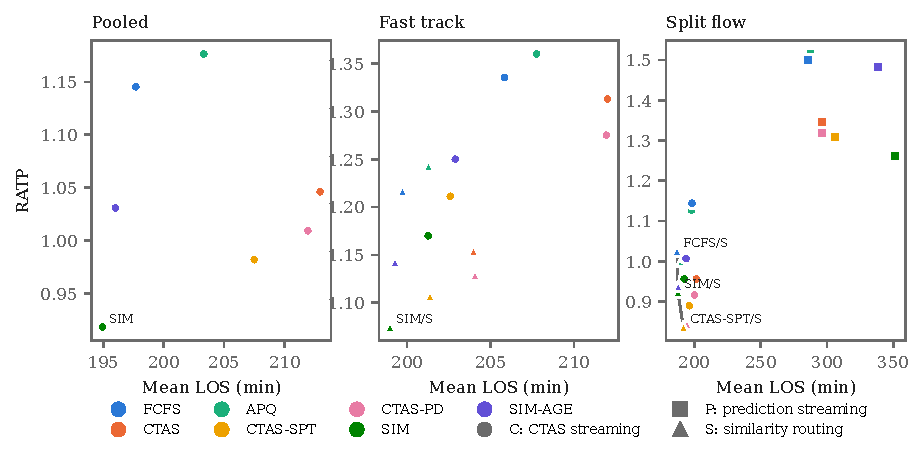
\includegraphics[width=\columnwidth]{figures/fig_pareto.pdf}
\caption{Mean LOS against RATP for all policies in the community ED at high load. Grey line: policies not dominated on both measures (labelled). Overloaded policies (Main-area utilization $\geq$ \OverloadThreshold) are omitted.}
\label{fig:pareto}
\end{figure}

Fig.~\ref{fig:pareto} shows the trade-off between RATP and mean LOS in the community ED at high load. In the pooled and fast-track configurations a single policy (SIM or SIM/S) is best on both measures; in split flow the non-dominated set contains several policies, and the choice depends on the weight given to access and flow. Fig.~\ref{fig:tails} and Table~\ref{tab:kpis} show the price of acuity-based ordering in the tails. In the pooled community ED at high load, the 95th percentile of door-to-physician time of CTAS~5 patients is \TailPNinetyFiveFcfsCtasFive{} hours under FCFS, \TailPNinetyFiveApqCtasFive{} hours under APQ, \TailPNinetyFiveSimCtasFive{} hours under SIM and \TailPNinetyFiveCtasCtasFive{} hours under CTAS. FCFS, in turn, lets the 95th percentile for CTAS~2 patients rise to \TailPNinetyFiveFcfsCtasTwo{} hours, against \TailPNinetyFiveCtasCtasTwo{} hours under CTAS. The ageing term of SIM-AGE shortens the CTAS~2 tail relative to SIM (\TailPNinetyFiveSimAgeCtasTwo{} against \TailPNinetyFiveSimCtasTwo{} hours) but not the CTAS~5 tail.

\begin{figure}[!t]
\centering
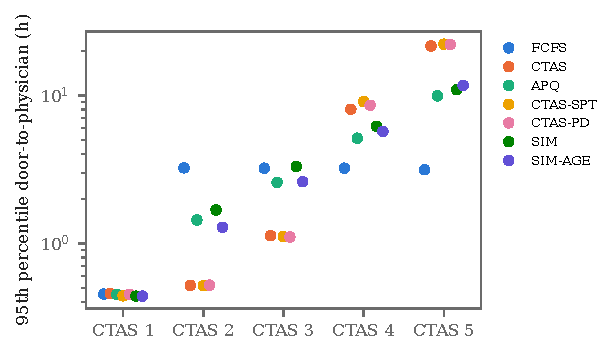
\includegraphics[width=0.95\columnwidth]{figures/fig_tails.pdf}
\caption{95th percentile of door-to-physician time by CTAS level and queue rule (community ED, high load, pooled; log scale).}
\label{fig:tails}
\end{figure}

\begin{table*}[!t]
\centering
\caption{Performance by queue rule in the community ED at high load (pooled; \Reps{} replications). Second line of each measure: paired difference from CTAS; bold if the 95\% confidence interval excludes zero.}
\label{tab:kpis}
\footnotesize
\begin{adjustbox}{max width=\linewidth}\begin{tabular}{lrrrrrrr}
\toprule
KPI & FCFS & CTAS & APQ & CTAS-SPT & CTAS-PD & SIM & SIM-AGE \\
\midrule
RATP & 1.145 & 1.046 & 1.177 & 0.982 & 1.009 & 0.918 & 1.031 \\
\quad vs CTAS & \textbf{+0.099} & -- & \textbf{+0.130} & \textbf{-0.064} & \textbf{-0.037} & \textbf{-0.128} & -0.015 \\
AWT (min) & 48.3 & 89.2 & 54.6 & 85.6 & 89.9 & 50.1 & 49.8 \\
\quad vs CTAS & \textbf{-41.0} & -- & \textbf{-34.6} & \textbf{-3.6} & +0.6 & \textbf{-39.1} & \textbf{-39.4} \\
P90 door to physician (min) & 147 & 206 & 164 & 152 & 185 & 102 & 150 \\
\quad vs CTAS & \textbf{-59} & -- & \textbf{-42} & \textbf{-53} & \textbf{-20} & \textbf{-104} & \textbf{-56} \\
P95 door to physician, CTAS 2 (min) & 194 & 31 & 86 & 31 & 31 & 101 & 77 \\
\quad vs CTAS & \textbf{+163} & -- & \textbf{+55} & -0 & +0 & \textbf{+70} & \textbf{+46} \\
P95 door to physician, CTAS 5 (min) & 188 & 1289 & 594 & 1328 & 1320 & 654 & 700 \\
\quad vs CTAS & \textbf{-1101} & -- & \textbf{-695} & +39 & +31 & \textbf{-635} & \textbf{-589} \\
Mean LOS (min) & 197.7 & 212.9 & 203.3 & 207.5 & 211.9 & 195.0 & 196.0 \\
\quad vs CTAS & \textbf{-15.2} & -- & \textbf{-9.6} & \textbf{-5.5} & \textbf{-1.0} & \textbf{-18.0} & \textbf{-16.9} \\
Mean LOS, discharged (min) & 160.9 & 184.1 & 170.2 & 176.8 & 179.7 & 146.3 & 156.8 \\
\quad vs CTAS & \textbf{-23.3} & -- & \textbf{-14.0} & \textbf{-7.3} & \textbf{-4.4} & \textbf{-37.8} & \textbf{-27.3} \\
Mean LOS, admitted (min) & 412.6 & 381.2 & 396.9 & 386.4 & 399.8 & 478.7 & 424.8 \\
\quad vs CTAS & \textbf{+31.4} & -- & \textbf{+15.7} & \textbf{+5.3} & \textbf{+18.7} & \textbf{+97.5} & \textbf{+43.6} \\
\bottomrule
\end{tabular}\end{adjustbox}
\end{table*}

\subsection{Value of Prediction Accuracy (RQ3)}

Fig.~\ref{fig:alpha} shows RATP as a function of the prediction error level $\alpha$ for the medium-load pooled and fast-track EDs, and Table~\ref{tab:vop} compares, for each of the \NMediumTypes{} medium-load ED types, the best policy that uses predictions with the best policy that does not (FCFS, CTAS or APQ, with CTAS streaming in two-area EDs).

\begin{figure*}[!t]
\centering
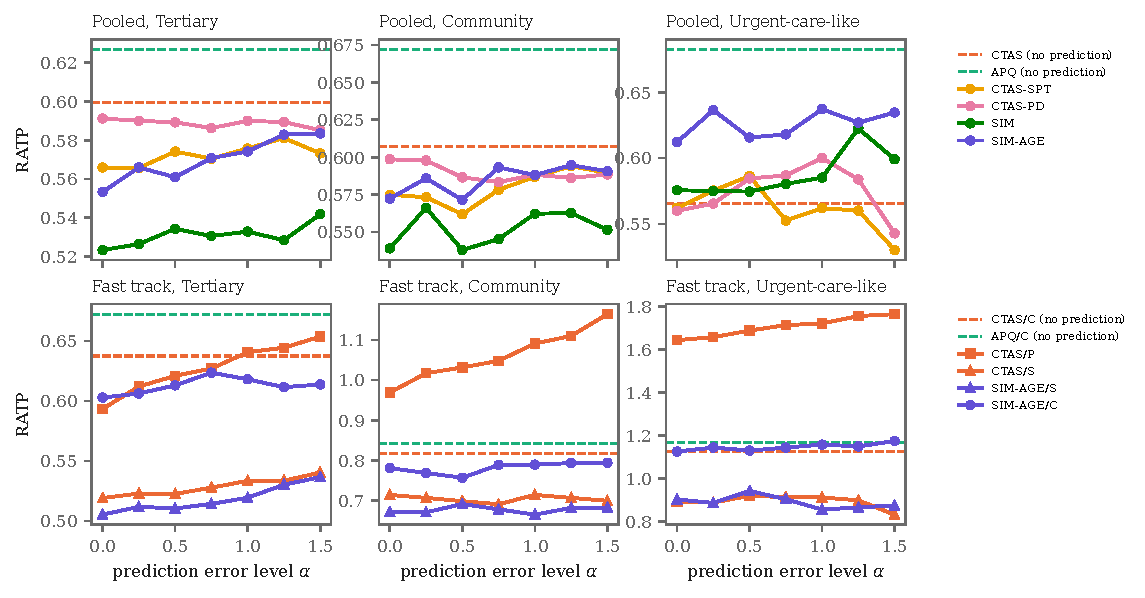
\includegraphics[width=0.9\textwidth]{figures/fig_alpha.pdf}
\caption{RATP against the prediction error level $\alpha$ ($\alpha=0$: perfect information; $\alpha=1$: reference accuracy) for medium-load pooled EDs (top, queue rules) and fast-track EDs (bottom, routing rules). Dashed lines: policies that do not use predictions. \RepsSecondary{} replications per point.}
\label{fig:alpha}
\end{figure*}

\begin{table*}[!t]
\centering
\caption{Gain of the best prediction-based policy over the best policy without predictions (medium load), with perfect information ($\alpha=0$) and reference accuracy ($\alpha=1$), and the largest $\alpha$ tested at which it is still better ($\geq$: better at every $\alpha$ tested).}
\label{tab:vop}
\footnotesize
\setlength{\tabcolsep}{2.5pt}
\begin{adjustbox}{max width=\linewidth}\begin{tabular}{llrrrrrr}
\toprule
 & & \multicolumn{3}{c}{RATP} & \multicolumn{3}{c}{Mean LOS} \\
\cmidrule(lr){3-5}\cmidrule(lr){6-8}
Acuity & Config. & Gain $\alpha{=}0$ (\%) & Gain $\alpha{=}1$ (\%) & Max $\alpha$ & Gain $\alpha{=}0$ (\%) & Gain $\alpha{=}1$ (\%) & Max $\alpha$ \\
\midrule
Tertiary & Pooled & 12.7 & 11.1 & $\geq$1.50 & 1.2 & 1.0 & $\geq$1.50 \\
 & Fast track & 23.3 & 21.5 & $\geq$1.50 & 3.6 & 3.3 & $\geq$1.50 \\
 & Split flow & 12.9 & 11.9 & $\geq$1.50 & 1.1 & 1.1 & $\geq$1.50 \\
Community & Pooled & 11.3 & 7.4 & $\geq$1.50 & 1.8 & 1.6 & $\geq$1.50 \\
 & Fast track & 21.2 & 20.9 & $\geq$1.50 & 0.8 & 0.8 & $\geq$1.50 \\
 & Split flow & 11.5 & 11.5 & $\geq$1.50 & 1.9 & 1.8 & $\geq$1.50 \\
Urgent-care-like & Pooled & 0.9 & 0.6 & 1.50 & 2.6 & 2.5 & $\geq$1.50 \\
 & Fast track & 22.4 & 25.9 & $\geq$1.50 & 2.6 & 5.0 & $\geq$1.50 \\
 & Split flow & 4.1 & 7.0 & 1.50 & 1.7 & 2.0 & $\geq$1.50 \\
\bottomrule
\end{tabular}\end{adjustbox}
\end{table*}

At the reference accuracy the best prediction-based policy had a lower RATP than the best policy without predictions in \VopNBetterAtOneRatp{} of the \NMediumTypes{} ED types and a lower mean LOS in \VopNBetterAtOneLosAllMean. The RATP gain ranged from \VopGainOneMinRatp\% to \VopGainOneMaxRatp\%; it was largest in fast-track EDs and smallest in the pooled urgent-care-like ED, where strict CTAS order is already close to the best. LOS gains were small, at most \VopGainOneMaxLosAllMean\%.

The gains depended little on prediction accuracy. From perfect information to the reference accuracy the RATP gain fell by \VopGainDropRatp{} percentage points on average, and the best prediction-based policy remained better than the best policy without predictions at every error level tested in \VopNAllAlphaRatp{} of the \NMediumTypes{} ED types for RATP and in \VopNAllAlphaLosAllMean{} for mean LOS. At the largest error level ($\alpha=\AlphaMax$) the exact-class accuracy of the service-time prediction is \AccSvcAtMax\%, no better than chance for five classes, and admission is predicted correctly for \AccAdmAtMax\% of patients. That the gains survive such poor predictions indicates that they come mainly from the structure of the rules, not from the information in the predictions. The queue rules remain anchored on the observed CTAS level, and similarity routing sends a larger share of patients to the second area whatever the predictions say (Section~\ref{sec:res:mech}).

Prediction streaming is the exception. It is the one rule in which predictions alone decide where a patient goes, and its RATP rose steadily with $\alpha$ and was worse than CTAS streaming at every error level in the community and urgent-care-like fast-track EDs (Fig.~\ref{fig:alpha}). In the tertiary fast-track ED it beat CTAS streaming when predictions were better than the reference accuracy, but not at the reference accuracy itself. For that rule accuracy matters, and in the other two fast-track EDs even perfect predictions did not make it competitive with the capacity split used here. The answer to how good predictions must be therefore depends on the rule: rules that use predictions to refine an acuity-based order tolerated large errors in our experiments, whereas the rule that streams patients on predictions alone was no better than CTAS streaming at the reference accuracy in any fast-track ED.

\subsection{Sensitivity to Boarding and Diagnostic Intensity}
\label{sec:res:sens}

Table~\aref{tab:sens} reports, for the \NMediumTypes{} medium-load ED types, whether the best policy of the core design remains the best when boarding is longer or diagnostic intensity changes (capacities unchanged), and how much is lost if the core best policy is kept. With light diagnostics the core best policy loses at most \SensLightDiagnosticsRatpRegretMax\% in RATP and \SensLightDiagnosticsLosAllMeanRegretMax\% in mean LOS. With high boarding the best policy for RATP changes in some ED types, but keeping the core best policy costs on average \SensHighBoardingRatpRegret\% in RATP (at most \SensHighBoardingRatpRegretMax\%) and \SensHighBoardingLosAllMeanRegret\% in mean LOS (at most \SensHighBoardingLosAllMeanRegretMax\%); the best queue rules are then \SensHighBoardingBestQueues. Long boarding hits split flow hardest, because admitted patients from the vertical area board in Main beds: in \SensHighBoardingNearSat{} ED types (\SensHighBoardingNearSatList) the median Main-space utilization across policies reached 0.95 or more.

Heavy diagnostics is the most demanding variant. In \SensHeavyDiagnosticsNearSat{} ED types (\SensHeavyDiagnosticsNearSatList) the median Main-space utilization across policies was 0.95 or more (up to \SensHeavyDiagnosticsUtilMax), because capacities were sized for typical diagnostic use. Close to saturation the core best policy lost up to \SensHeavyDiagnosticsLosAllMeanRegretMax\% in mean LOS; elsewhere it held up, which suggests that the results are least reliable for an ED operating close to the capacity of its Main area.




\subsection{A Decision Guide}

Table~\ref{tab:guide} condenses the results into a guide for ED managers. For each acuity mix and configuration it gives the policy with the smallest mean regret over the three load levels, separately for access (RATP), flow (mean LOS) and their average, with the largest regret over the load levels. Within an acuity mix and configuration, a single policy is within \GuideMaxRegretRatp\% of the best RATP and within \GuideMaxRegretLos\% of the best mean LOS at every load level, so the load level matters less for the choice than the acuity mix and the configuration. A classification tree fitted to the best queue rule by ED type confirms this ordering: it splits first on acuity mix and then on configuration, and with \TreeRatpLeaves{} leaves it reproduces the best queue rule for RATP in \TreeRatpAcc\% of the ED types.

\begin{table*}[!t]
\centering
\caption{Decision guide: recommended policy by acuity mix and configuration (smallest mean regret over the three load levels) and the largest regret over the load levels. ``Balanced'' uses the average of the RATP and mean-LOS regrets.}
\label{tab:guide}
\footnotesize
\begin{adjustbox}{max width=\linewidth}\begin{tabular}{llrlrlr}
\toprule
 & & \multicolumn{2}{c}{Access (RATP)} & \multicolumn{2}{c}{Flow (mean LOS)} & \multicolumn{1}{c}{Balanced} \\
\cmidrule(lr){3-4}\cmidrule(lr){5-6}\cmidrule(lr){7-7}
Acuity mix & Configuration & Policy & Max regret (\%) & Policy & Max regret (\%) & Policy (max regret, \%) \\
\midrule
Tertiary & Pooled & SIM & 0.0 & SIM & 0.0 & SIM (0.0) \\
 & Fast track & SIM/S & 0.0 & SIM/S & 0.1 & SIM/S (0.0) \\
 & Split flow & SIM/S & 0.0 & SIM/S & 0.1 & SIM/S (0.0) \\
Community & Pooled & SIM & 0.5 & SIM & 0.0 & SIM (0.3) \\
 & Fast track & SIM/S & 0.0 & SIM/C & 1.2 & SIM/S (1.8) \\
 & Split flow & CTAS-SPT/S & 0.0 & FCFS/S & 0.3 & CTAS-SPT/S (1.3) \\
Urgent-care-like & Pooled & CTAS-SPT & 1.9 & SIM & 0.0 & CTAS-SPT (4.5) \\
 & Fast track & SIM/S & 1.2 & SIM/S & 0.1 & SIM/S (0.6) \\
 & Split flow & CTAS/S & 2.5 & FCFS/S & 0.0 & CTAS/S (2.4) \\
\bottomrule
\end{tabular}\end{adjustbox}
\end{table*}
